\documentclass[11pt]{article}
\usepackage{lmodern}
\usepackage{amssymb,amsmath}
\usepackage{ifxetex,ifluatex}
\usepackage{fixltx2e} % provides \textsubscript
\ifnum 0\ifxetex 1\fi\ifluatex 1\fi=0 % if pdftex
  \usepackage[T1]{fontenc}
  \usepackage[utf8]{inputenc}
\else % if luatex or xelatex
  \ifxetex
    \usepackage{mathspec}
    \usepackage{xltxtra,xunicode}
  \else
    \usepackage{fontspec}
  \fi
  \defaultfontfeatures{Mapping=tex-text,Scale=MatchLowercase}
  \newcommand{\euro}{€}
\fi
% use upquote if available, for straight quotes in verbatim environments
\IfFileExists{upquote.sty}{\usepackage{upquote}}{}
% use microtype if available
\IfFileExists{microtype.sty}{%
\usepackage{microtype}
\UseMicrotypeSet[protrusion]{basicmath} % disable protrusion for tt fonts
}{}
\ifxetex
  \usepackage[setpagesize=false, % page size defined by xetex
              unicode=false, % unicode breaks when used with xetex
              xetex]{hyperref}
\else
  \usepackage[unicode=true]{hyperref}
\fi
\usepackage[usenames,dvipsnames]{color}
\hypersetup{breaklinks=true,
            bookmarks=true,
            pdfauthor={},
            pdftitle={},
            colorlinks=true,
            citecolor=blue,
            urlcolor=blue,
            linkcolor=magenta,
            pdfborder={0 0 0}}
\urlstyle{same}  % don't use monospace font for urls
\usepackage{longtable,booktabs}
\usepackage{graphicx,grffile}
\makeatletter
\def\maxwidth{\ifdim\Gin@nat@width>\linewidth\linewidth\else\Gin@nat@width\fi}
\def\maxheight{\ifdim\Gin@nat@height>\textheight\textheight\else\Gin@nat@height\fi}
\makeatother
% Scale images if necessary, so that they will not overflow the page
% margins by default, and it is still possible to overwrite the defaults
% using explicit options in \includegraphics[width, height, ...]{}
\setkeys{Gin}{width=\maxwidth,height=\maxheight,keepaspectratio}
\setlength{\parindent}{0pt}
\setlength{\parskip}{6pt plus 2pt minus 1pt}
\setlength{\emergencystretch}{3em}  % prevent overfull lines
\providecommand{\tightlist}{%
  \setlength{\itemsep}{0pt}\setlength{\parskip}{0pt}}
\setcounter{secnumdepth}{0}

\date{}

% Redefines (sub)paragraphs to behave more like sections
\ifx\paragraph\undefined\else
\let\oldparagraph\paragraph
\renewcommand{\paragraph}[1]{\oldparagraph{#1}\mbox{}}
\fi
\ifx\subparagraph\undefined\else
\let\oldsubparagraph\subparagraph
\renewcommand{\subparagraph}[1]{\oldsubparagraph{#1}\mbox{}}
\fi

\setlength{\oddsidemargin}{-0.1in}
\setlength{\topmargin}{-0.52truein} 
\setlength{\textheight}{9.15in} 
\setlength{\textwidth}{6.7in}

\usepackage[T1]{fontenc}
\usepackage{fourier}
\usepackage[sc]{mathpazo}
\linespread{1.05}         % Palatino needs more leading (space between lines)


\usepackage{wrapfig}
\usepackage[square,numbers,sort&compress]{natbib}
\renewcommand{\cite}{\citep}
%\usepackage[psamsfonts]{amssymb}
%\usepackage{palatino}
%\usepackage{mathpazo}
\usepackage{plasmadefs}

\hyphenation{wave-packet wave-packets}

\title{}

\begin{document}

\section{Introduction and Motivation}

This renewal proposal requests funds to continue operation of the Basic
Plasma Science Facility (BaPSF) at the University of California, Los
Angeles (UCLA), and to support the vigorous research program of the
BaPSF scientific staff, as well as to continue the improvements in
scientific instrumentation required to maintain worldwide leadership in
fundamental plasma research.  BaPSF provides national and international scientists access to unique
research devices and diagnostic tools that permit the exploration of a
wide range of fundamental plasma problems that impact topics at the
frontiers of fusion, space science and plasma technology. The broad
parameter ranges accessible in the plasma devices operated at BaPSF
allow studies that span microscopic phenomena on the fast electron time
scales (e.g., electron plasma waves, cyclotron radiation) to the slow
time scales characteristic of plasma transport driven by drift-wave
turbulence and long wavelength magnetic fluctuations. This extensive
basic plasma research capability in a single laboratory setting is not
available anywhere else, but examples of analogous user facilities exist
in other scientific disciplines. Qualified researchers and research
teams from universities, national laboratories and industry can perform
experiments at BaPSF, free of charge, upon approval of their proposals
by a Scientific Council composed of senior scientists broadly
representative of the plasma community.

Over the past 5 years, the scientific activities at BaPSF involve
individuals affiliated with 18 different institutions: 11 professors,
12 Ph.D. scientists, 15 graduate students and 12 undergraduate
students.  The research modalities accommodate a range of options:
single-user operation, theory-driven investigations, and topical
campaigns. Single users consist of small groups who pursue a
well-defined theme that can be brought to a successful completion
without major involvement from the BaPSF scientific
staff. Theory-driven studies involve important problems suggested by
individuals who are not directly qualified to perform experiments in a
complex hardware environment, but who define the scientific goals and
participate in the data gathering, analysis and interpretation of
experiments conducted by the BaPSF staff. This mode requires extensive
support by the BaPSF scientific and technical staff and often involves
UCLA graduate students. Topical campaigns consist of a large and
diverse group of researchers from various institutions who pursue a
common set of problems of contemporary interest. The campaigns involve
experimentalists, theoreticians, modelers, and also the BaPSF
scientific and technical staff. Over the past (five year) funding
cycle these various modes of operation have resulted in 46 reviewed
publications and 39 invited presentations (listed in Appendix)
Selected highlights from these studies are presented later.

The BaPSF plasma devices provide effective platforms for the training
of graduate students because of their optimum, mid-scale size. The
devices and diagnostic tools available at the BaPSF are sufficiently
large and sophisticated so as to provide exposure to frontier
developments that require learning to work in a team
environment. These are valuable experiences not commonly available to
graduate students in small, single-PI laboratories. Yet, the size of
the BaPSF operation is small enough for students to obtain individual
hands-on experience not available at facilities with large fusion
devices. Over the past funding cycle, 11 students have earned Ph.D.s
based on work performed at the BaPSF, and 3 have completed
M.S. degrees.

The reliable and flexible operation of the BaPSF, by a dedicated and
experienced staff, also provides a fertile environment for the
development of young faculty by allowing them to focus entirely on
scientific research. Over the past funding cycle, Prof. C. Niemann
(UCLA) performed experimental studies at BaPSF that culminated in his
receiving tenure. Prof. G. Howes (U. Iowa) also received tenure during
this period with a research portfolio that included BaPSF experiments.
Currently, J. Bortnik (UCLA) is taking advantage of the BaPSF to develop
a similar career trajectory. It is expected that other young faculty
members will similarly benefit from the BaPSF capabilities during the
next 5 years of operation.

An essential element leading to the successful operation of BaPSF is the
vigorous research program pursued by the scientific staff of the
facility. The results obtained by these researchers expand the frontiers
of the field, explore the limits of the hardware, and pave new avenues
for BaPSF users to pursue. A scientific research program led by the BAPSF staff is part of
this proposal.  

Our vision for the future of BaPSF is to create a facility with enough
flexibility to address frontier scientific issues that cut across
multiple disciplines within plasma science. Such issues as; Alfvénic
shocks, 3D reconnection, turbulence and transport, radiation belt
physics, solar and stellar wind turbulence, and solar atmospheric
transport and turbulence. We plan to accomplish this by providing a
range of well-diagnosed research devices than span a parameter space
of sufficient breadth to address many problems of current interest, an
infrastructure that allows easy and interchangeable access to all
devices, and a management structure that promotes cooperation between
experimentalists, theoreticians and computer modelers.

\section{Organization and Operation}

Currently the BaPSF operates five plasma devices having complementary
capabilities that meet different research, development and educational
needs of the user community. The centerpiece is the Large Plasma Device
(LAPD). The LAPD generates highly reproducible and quiescent magnetized
plasma columns 18 meters in length, once per second, over a continuous
period of approximately three months. Details of the operational parameters are given in the Appendix
(table A1). This linear device has been in operation for nearly 20 years
and undergoes continuous improvements to provide the world's
most advanced research tool for basic plasma science. This is the
primary device used in implementing
the facility research programs. An upgrade to the LAPD is planned as
part of the proposed work, adding a new plasma source that will increase
uptime and significantly expand the range of plasma parameters
accessible using the device. The Small Plasma Device (SMPD) is a
low-field plasma chamber four meters in length used to develop probes,
test new diagnostic concepts, and perform research on topics that do not
require the high-performance plasma parameters available in the LAPD.
The Enormous Toroidal Plasma Device (ETPD) is a large, toroidal plasma
chamber with a major radius of 5 meters in development as a research
tool. The ETPD is presently used to test new cathode concepts for
generating long, high-density plasma columns, and is potentially of
great interest to fusion, space, solar and astrophysical researchers.
Over the past 5 years, a graduate student is completed a Ph.D.
dissertation related to the plasma processes involved in the formation
of the ETPD plasma column. A plasma processing device, donated by
industry, provides a platform for the study of low temperature plasmas
and the properties of RF sheaths. Two graduate students have used this
tool to complete Ph.D. studies related to the energetic ion distribution
functions formed in these environments. The diagnostics and experience
obtained using this tool will be beneficial in a forthcoming campaign
related to RF antennas used in fusion plasmas. Finally, a small,
dedicated machine with a helicon-generated plasma is used to train high
school teachers and students enrolled in the LAPTAG (Los Angeles
Physics Teachers Alliance Group) outreach program~\citep{laptag}.
Work done in this device by the high school students and teachers is
routinely presented at meetings and some results have been published.

During the last funding cycle LAPD operated in a reliable, steady-state
research mode. On average, the machine was available for scientific
research over 70 percent of the time, exceeding the target of 60 percent
availability set in the original facility proposal. On average, over the
last three years (2012-2014) the LAPD was available 282 days out of the
year (80\% uptime). Maintenance (primarily the periodic replacement of
the Barium Oxide cathode coating) accounted for 14\% of the downtime. Of
the 282 days of operation, 64\% of the run time was allocated to
external users with the remaining 36\% allocated to the local group; the
original facility proposal dictated a 50-50 split between external
users and the local group.

\subsection{Management Structure}

The goal of facility management is to maximize scientific productivity
while providing users dependable and convenient access to all facility
resources. For management purposes facility users are divided into two
groups: the local group and external users. For this renewal proposal,
the local group consists of four BaPSF Principal Investigators: T.
Carter, W. Gekelman, G. Morales, and S. Vincena together with the
postdoctoral scientists and graduate students associated with their
research. External users are all other researchers, including those
resident at UCLA, who have no responsibility for BaPSF operations.

For this renewal, BaPSF will led by a director, Troy Carter, who will
be responsible for the operation of the facility and supervision of
facility personnel, the overall coordination of the interaction with
the user groups, and reporting to funding agencies. Walter Gekelman
had been director of BaPSF since its inception in 2000 and led the
team that designed and constructed the LAPD device. For the proposed
renewal period, Prof. Gekelman will take on the role of Associate
Director for Project Development and will lead hardware development
for the facility, in particular the major cathode upgrade project
described below. Dr.  Vincena helps the director coordinate facility
use with the efforts of the local research group and is responsible
for the generation of reliable plasma conditions in
LAPD. Prof. Morales oversees the connection of the facility
experimental program to the broad plasma science community and
monitors the overall scientific directions. The director is assisted
by a staff consisting of a technical coordinator and scientific
liaisons. The technical coordinator (Zoltan Lucky) is responsible for
the overall maintenance of the plasma devices and laboratory
equipment, including probes, probe drives and electronics.  The
scientific liaisons (Drs. Bart Van Compernolle and Shreekrisna
Tripathi) assist external users in operating the LAPD and in
implementing their experimental objectives. The facility has a full
time Project Scientist/Engineer (Dr. Pat Pribyl), three full time
laboratory technicians and an administrative assistant.

\subsection{Facility Access}

Individuals interested in performing experiments at the facility
submit a short white paper to the director outlining a proposed
experiment. The director consults with the local group concerning the
feasibility of implementing the proposed experiment. The director
reserves the right to refuse any experiments deemed likely to cause
irreparable or significant damage to the infrastructure. For each
feasible experiment, the director obtains an evaluation of the
scientific quality and recommendation of the priority of the proposed
experiment from the Scientific Council. For each approved white paper,
the director assigns a scientific liaison to be the contact person
with the proposer. Most external users submit proposals to the funding
agency of their choice where they are reviewed according to the
individual procedures of the agency. The scientific liaison aids in
supplying any information needed to write a full proposal. The
director includes a letter of support and a commitment to provide the
machine time needed for the proposed experiment. Some users already
have funding or do not require support, and thus proceed to access
BaPSF resources directly upon approval.

When a user group arrives at the facility to conduct an experiment, they
interface with the assigned scientific liaison. The liaison assists the
user group with the use of facility assets in order to insure the safety
of personnel, and to protect facility resources from improper use. The
scientific liaison makes sure that the necessary facility equipment and
diagnostics are available and operational at the required time, assists
in the preparations for data acquisition and is on the floor with the
user team to aid in the successful implementation of the research plan.
After experimental data is acquired the liaison assists, if requested by
the users, in local visualization and analysis of data, exportation of
data and data backup.

\subsection{Scientific Council}

The scientific council gives advice and guidance to the BaPSF PIs on
management and scientific issues. The council meets formally at the
annual APS-DPP meeting to review progress, suggest improvements, and
provide advice to the director concerning policy matters. Through email
communications, the council reviews white papers and makes a
recommendation to the director on granting facility access. The current
membership of the council is: R. Berger (LLNL), B. Briezman (U. Texas),
V. Chan (General Atomics), M. Koepke (WVU), S. Spangler (U. Iowa), and
E. Zweibel (U. Wisconsin). Dr. Chan has recently retired from GA and
will be cycling off the council. Normally, council membership is
refreshed approximately every year by rotating out one member. New
members are selected by the PIs upon the advice of the council and in
consultation with the funding agencies. On July 20, 2015 the council
visited UCLA to examine the status of the facility hardware and
infrastructure, and to give advice on the preparation of this proposal.


\subsection{Users Group}

A BaPSF users group was created over the prior funding period with the
following goals: (1) provide a forum for users to \ldots{}.

{Discuss leadership, list meetings, point to appendix for recent users
group report}


\section{Results from Prior Support}

In this section we present highlights of selected research programs from
both the external user groups and the local group. Details of research
programs not covered here are included in the Appendix.  

\subsection{Research Highlights -- External user groups:}

Over the past 5 years, there have been six independent experimental user
groups, seven theory-driven studies and three topical campaigns. The
leaders of these various efforts and their affiliated institutions are
listed here; highlights from 5 of these research programs follow.

\begin{description}
\item{\emph{Independent experimental user groups}}: 1) W. Heidbrink
(University of California, Irvine); 2) C. Niemann (UCLA); 3) C. Kletzing, F. Skiff, G. Howes (University of Iowa); 4) M.
Koepke (West Virginia University); (5) D. Bui, Y. Song (Tri Alpha
Energy); (6) J. Judy (UCLA)

\item{\emph{Theory-driven studies}}: 1) P. Colestock. M. Light (LANL);
2) J. Bortnik, R. Thorne (UCLA); 3) W. Daughton, J. Finn (LANL); (4) M.
Kushner (U. Michigan); (5) D. D'Ippolito, J. Myra (Lodestar Corp); (6)
A. Streltsov (Embry-Riddle University); (7) Li-Jen Chen (U. New
Hampshire).

\item{\emph{Campaigns}}: 1) ``Fast-Ion Campaign'', W. Heidbrink
(University of California, Irvine ); 2) ``Auroral Physics Campaign'', M. Koepke (West Virginia Univ.); 3)
``Radiation-belt Physics Campaign'', D. Papadopoulos, T. Antonsen (University of Maryland).
\end{description}



\subsubsection{Generation of an Alfv\'{e}nic shock
using a high power laser  (C. Niemann, C. Constantin, W. Gekelman,
S. Vincena; A. Bondarenko, D. Schaeffer, E. Everson (grad students) (UCLA))}

Magnetosonic collisionless shocks have been driven using an exploding
laser-produce plasma in LAPD~\citep{schaeffer:2014,niemann:2014}. This is the very first
observation of collisionless shocks of cosmic relevance in a large,
current-free laboratory plasma and the first experimental measurement
of the shock formation time.

In these experiments a plastic target was irradiated with an energetic
200J laser beam from the new high-energy glass laser. A blow-off plasma
was created that exploded at super-Alfvenic speed into an
H\textsuperscript{+} ambient plasma perpendicular to the 300 G external
field.

\begin{figure}[!htbp]
\centerline{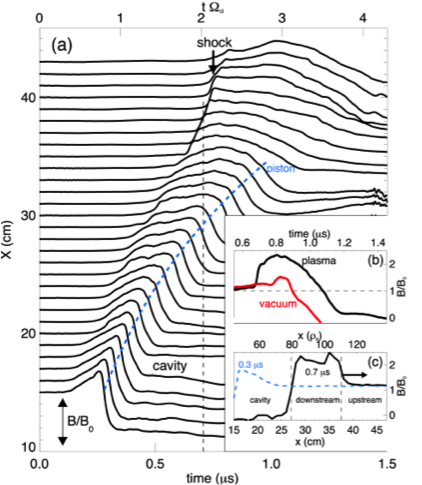
\includegraphics[width=3.0truein]{shock1}}
\caption{a) Magnetic stack plots of $B_{z}$ as a function of time for
  various distances from the target. (b) Comparison of $B_z(t)$ at $x
  = 35$cm with (black) and without (red) the ambient plasma. (c) Structure
  of the pulse before ($t = 0.3$ $\mu$s) and after a shock is formed.}\label{shock1}
\end{figure}

Figure~\ref{shock1}(a) shows stack plots of the measured magnetic field
$B_z/B_o$ for various
distances $x$ from the laser target. Each trace shows the typical
signature of a diamagnetic laser plasma cavity, including an initial
field compression followed by complete field expulsion. The magnetic
pulse ahead of the cavity travels at $370 \pm 20$ km/s, which is
super-Alfvénic ($M_A = 2.2 \pm 0.3$). The magnetic
piston, i.e., the leading edge of the diamagnetic cavity, slows from
500~km/s near the target to 200~km/s in the center of the vessel. About 20~cm from the target, corresponding to
$t \Omega_{i} =1$, the magnetosonic pulse starts to
steepen into a shock and to separate from the piston. The ramp continues
to steepen up to a distance of 40~cm from the target, at which point the
ambient plasma density drops sharply, and the shock dissipates. The
measured field compression of $B_z/B_o \ge 2$ is consistent
with the Rankine-Hugoniot jump conditions for a shock. In comparison
with expansion into vacuum (Figure~\ref{shock1}(b)), the field compression is
significantly larger with the ambient plasma and the leading edge of the
magnetic pulse expands faster, indicating that the pulse is carried by
ambient ions, which have been accelerated by the piston. Simultaneously,
the trailing edge of the pulse (i.e., the piston) moves much slower,
indicative of energy transfer to the ambient plasma. The magnetic pulse
in vacuum has a significantly shallower ramp due to fast ions that slip
through the magnetic field, causing a weak magnetic disturbance ahead of
the pulse. The spatial profile (Figure~\ref{shock1}(c)) shows a ramp with a width of
a few millimeters and a downstream region between the piston and the
ramp of 30 ambient ion gyroradii. In comparison to earlier times before
the shock is formed (blue dashed line in Figure~\ref{shock1}(c)), the structure of
the shock shows a significantly steeper and faster ramp, and a much
broader, more compressed pulse. In addition, the ramp of the shock
steepens from an initial 40 $c/\omega_{\rm pe}$ to less
than 20 $c/\omega_{\rm pe}$ at a distance of 40 cm from
the target. The measured shock formation time around
$t \Omega_{i} = 1$ is consistent with theoretical
predictions, while the measured coupling parameter of
$R_M/\rho_d = 1 \pm 0.1$ agrees
well with the requirements found in hybrid simulations~\cite{clark:2014}.


\subsubsection{Resonant interactions between energetic electrons and whistler
waves (J. Bortnik, R. Thorne, B. Van Compernolle; X. An (Graduate
Student) (UCLA))}


A major scientific problem of current interest is the determination of
the dominant physical processes that drive the dynamic variability of
the outer radiation belt \cite{thorne:2010, reeves:2013}. Resonant interactions between
energetic electrons and whistler mode waves are thought to play an
essential role~\cite{horne:2005, thorne:2013}. The ongoing theory-driven
LAPD project, led by J. Bortnik, has a two-pronged approach; the
resonant scattering of energetic electrons by whistler waves~\cite{vancompernolle:2014} is studied as well as the excitation of
whistler waves by energetic electrons. The experimental work has been
made possible by the development of a 10 cm diameter energetic electron
beam source, with beam energies up to 5 keV.

\begin{figure}[!htbp]
\centerline{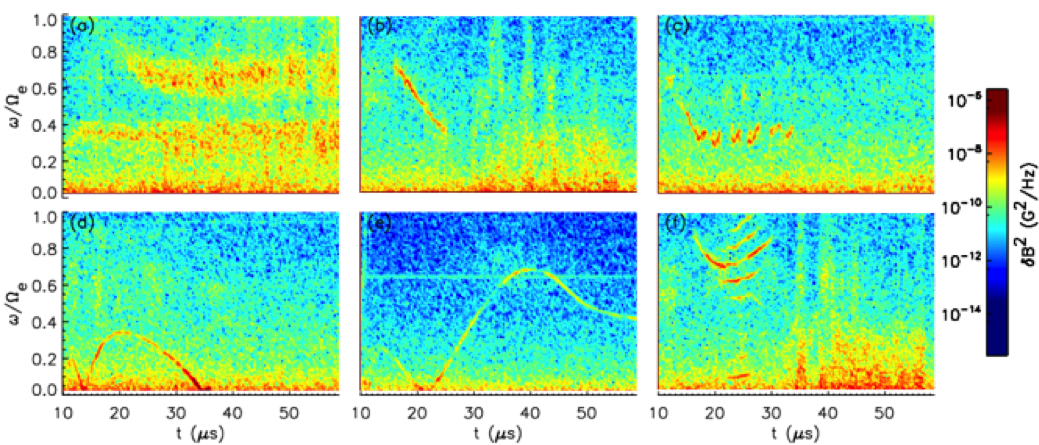
\includegraphics[width=5.0truein]{bortnik1}}
\caption{Examples of spectrograms of whistler wave excitation. (a)
  broadband waves, (b) falling tone, (c) multiple consecutive chirps,
  (d) double hook, (e) long rising and falling tone, (f) chirps at
  multiple frequencies simultaneously}\label{bortnik1}
\end{figure}


In the past two years the experiment has focused on the excitation of
whistler waves by energetic electrons under various plasma and beam
conditions. A very recent result~\cite{vancompernolle:2015a} is the excitation
of discrete frequency chirping whistler waves, which have been observed
in space for decades known as chorus waves, but have up to now never
been observed in the laboratory. The experiment identifies stringent
conditions under which the discrete frequency chirping is seen. There is
a strong dependence on beam density, plasma density and the guide field
profile and magnitude. Examples of the rich variety of beam-generated
wave activity is displayed in the spectrograms in Fig.~\ref{bortnik1}. The
experiment allows, for the first time, to test under controlled
conditions the leading theories in nonlinear whistler wave excitation.
Manuscripts are also being prepared on the excitation of broadband
whistler waves (non-chirping). It is shown that energetic electrons
resonantly excite whistler waves simultaneously through the Doppler
shifted cyclotron resonance, the Cherenkov resonance as well as through
the anomalous cyclotron resonance, i.e. through the relation $\omega -
k_\parallel v_{{\rm beam}, \parallel} = n\Omega_{e}$ where
$n=1,0,-1$. Comparisons with
growth rate calculations show excellent agreement with the
experiment.  Graduate student X. An will present an invited talk on
this work at the upcoming APS DPP meeting in Savannah, GA.

\subsubsection{Fast-ion Campaign (W. Heidbrink, R. McWilliams (UC Irvine), B.
Breizman (UT Austin), F. Jenko (MPI Garching/UCLA), S. Tripathi, S.
Vincena, T. Carter (UCLA))}

The campaign led by Prof. W. Heidbrink (UCI) is focused on the basic
physics of the interaction between energetic ions and collective modes
supported by a magnetized plasma. It is motivated by the need to
understand the complex behavior of alpha particles in a burning,
magnetically confined plasma.

A recent campaign highlight is the investigation of the interaction
between fast ions and drift-wave turbulence in LAPD. 

\subsubsection{Alfvèn wave-wave interactions relevant to MHD turbulence (G.
Howes, F. Skiff, C. Kletzing (U. Iowa); T. Carter, S. Dorfman (UCLA))}

{[}To be added\ldots{}{]}

\subsubsection{Radiation Belt Remediation (Campaign) (Dennis Papadopoulos, Tom
Antonsen (Univ. Maryland), Yuhou Wang, W. Gekelman, P. Pribyl, G.
Morales (UCLA))}

Laboratory observations of enhanced loss of magnetic mirror trapped fast
electrons irradiated by a shear Alfv\'{e}n Wave (SAW) are reported. A
trapped energetic electron population ($> 100$keV) is
generated in a magnetic mirror section (mirror ratio $\approx$ 2,
length = 3.5
m) by an X-mode high power microwave pulse, and forms a hot electron
ring due to the grad-B and curvature drift. SAWs of arbitrary
polarization are launched externally by a Rotating Magnetic Field (RMF)
source ($\delta B/B_o \approx 0.1$\%, $\lambda_\parallel \approx 9$m).
Irradiated by a right-handed circularly polarized SAW, the loss of
electrons, in both the radial and the axial direction of the mirror
field, is significantly enhanced and is modulated at
f\textsubscript{Alfv\'{e}n}. The periodical loss continues even after the
termination of the SAW. Experimental observations suggest that a spatial
distortion of the ring is formed in the SAW field and creates a
collective mode of the hot electron population that degrades its
confinement and leads to electron loss from the magnetic mirror.

The hot electron ring was produced using a magnetron ($f=2.45$ GHz)
coupled to the plasma with a circular waveguide. The microwaves were
resonant with electrons at the second cyclotron harmonic (400G  near
the center of the magnetic mirror). A shear Alfv\'{e}n wave launched with a
rotating magnetic field antenna (located outside of the mirror)
de-trapped all electrons in a wide energy range (100 eV \textless{}
E\textless{}3 MeV). Evidence of SAW effectively de-trapping the hot
electron population is found in the x-ray flux measurement when the
trapped electrons are further accelerated to energies that enable hard
x-ray production~\cite{wang:2012}. Shown in Fig.~\ref{muri1} are
traces E-J, showing  that a burst of x-rays
generated by hot electrons escaping the mirror trap and striking
metallic surfaces appears during the Alfv\'{e}n wave propagation time. A
large flux of x-ray appears while the Alfv\'{e}n wave is first turned on.
After this initial burst, the x-ray flux decreases as the remaining hot
electron population is depleted during the rest of the Alfv\'{e}n on time.
After the Alfv\'{e}n wave is turned off, the x-ray flux slowly builds up due
to the presence of ECRH which remains on until $t = 30$ ms.

\begin{figure}[!htbp]
\centerline{
\includegraphics[width=3.5truein]{muri1}}
\caption{Time series of x-ray flux
measured by an un-collimated detector, designated by letters A-T. The
ECRH is on from t=0 to 30 ms, but only after about 20 ms are there
sufficient high energy electrons to produce a measurable x-ray flux.
Trace A is measured without launching the SAW. In traces B-T a 100 cycle
shear Alfvén wave pulse (total duration = 0.87 ms), starting at
different times labeled on the graph is launched. Each trace is averaged
over 50 plasma shots.}\label{muri1}
\end{figure}

After the ECRH terminates at $t = 30$ ms, a population of fast electrons
persists in the mirror, and can be de-trapped by launching Alfvén waves
at these late times, as evidenced by x-ray bursts in Fig.~\ref{muri1} traces K-T.
The estimated trapping time for a 200~keV electron is 40~ms before its
loss from cumulative collisions with the helium atoms and ions. The
decay of the x-ray burst intensity after $t = 31$~ms reflects the decay of
the number of x-ray producing hot electrons still in the mirror. This
measurement proves that the electron loss due to the shear Alfvén wave
is not related to the presence of the microwaves. An X ray tomography
system was developed to establish here the hot electrons go after having
interacted with the wave~\cite{wang:2013}. Most of the fast electrons strike the
waveguide, which is very close to the plasma edge. Electrons are also
lost of a mesh anode at the end of the device. These have been scattered
out of the loss cone~\cite{wang:2014}.




\subsection{Local group research}

\subsubsection{From heat transport in LAPD to chaotic fluctuations in DIII-D (J.
Maggs, G. Morales)}

An unexpected research path has lead to a connection between basic heat
transport experiments in LAPD to the identification that the density
fluctuations in the L-mode plasmas in the DIII-D tokamak are chaotic. To
simplify the study of electron heat transport, a series of basic
experiments have been performed in LAPD. The generic experiment uses a
small (3mm diameter), single-crystal LaB\textsubscript{6} cathode to
inject a low-voltage electron beam into a strongly magnetized (1 kG),
cold, afterglow-plasma. The low-voltage beam acts as an ideal heat
source that produces a long ($\sim$8 m), narrow ($\sim$5mm in radius) temperature
filament that is well separated from the walls of the machine. The
existence of a transition from a regime of classical transport to one of
anomalous transport has been established through detailed measurements.
During the period of classical transport, drift-Alfvén waves grow
linearly, driven by the temperature gradient. To elucidate the dynamics
leading to anomalous transport the permutation entropy analysis (C-H
plane technique) developed by \citep{rosso:2007} is applied to the
probe signals. This technique is an effective method to identify the
various possible dynamical processes (coherent, stochastic, chaotic,
fractional Brownian motion). In a characteristic C-H display, the
vertical axis corresponds to the Jensen-Shannon complexity, C, and the
horizontal axis to the normalized Shannon entropy, H. These quantities
are obtained from the Bandt-Pompe probability distribution~\cite{bandt:2002}
generated from the time series. Through these techniques it has been
conclusively shown that the LAPD anomalous heat transport is a
consequence of chaotic dynamics~\cite{pace:2008,maggs:2012a,maggs:2012b,maggs:2013}. Motivated by this finding a
collaboration was established with Dr. T. Rhodes who performs very
delicate Doppler-backscattering (DBS) measurements of the fluctuations
in the DIII-D tokamak. The analysis methodology developed for the LAPD
was applied to the DIII-D and it was found that the behavior of the
fluctuations in that seemingly different experiment exhibit the same
chaotic behavior as the simple LAPD experiment~\cite{maggs:2015}.

\begin{figure}[!htbp]
\centerline{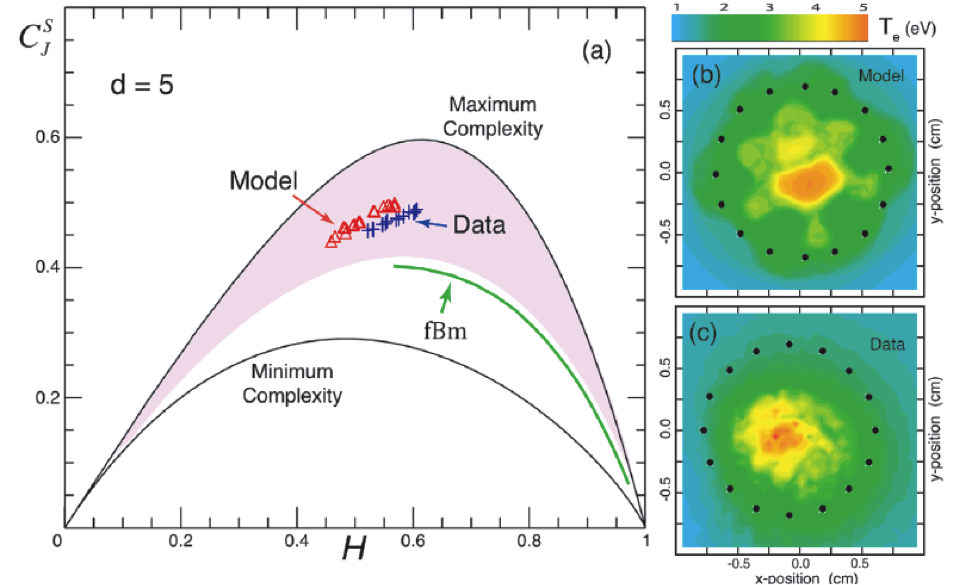
\includegraphics[width=3.8truein]{chaos1}}
\caption{C-H plane analysis of data in LAPD experiment and of prediction
of a chaotic advection model shows LAPD dynamics are chaotic.}\label{chaos1}
\end{figure}

\begin{figure}[!htbp]
\centerline{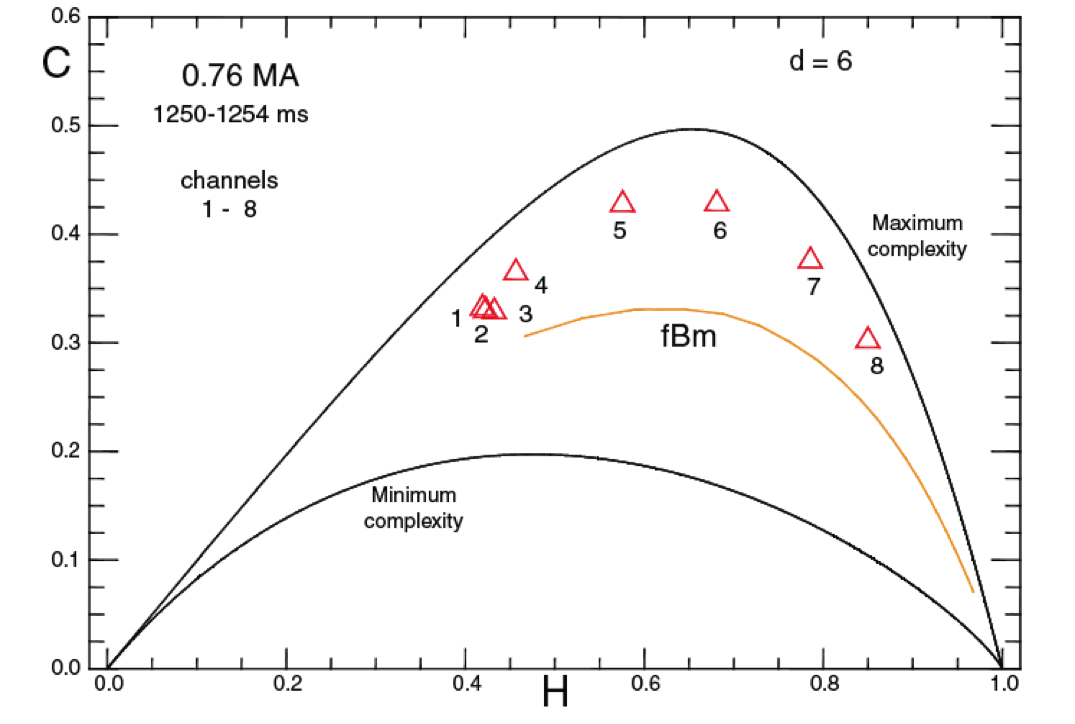
\includegraphics[width=3.8truein]{chaos2}}
\caption{C-H plane analysis of Doppler-backscattering (DBS) from DIII-D
shows that the signals from all the channels (different radii) are in
the chaotic region, as in the LAPD experiment.}\label{chaos}
\end{figure}


\subsubsection{Ion-ion hybrid Alfvén wave resonator (S. Vincena, G. Morales, J.
Maggs)}

A detailed experimental and theoretical investigation has firmly
established the reality of a wave resonator based on the concept of wave
reflection along the confinement magnetic field at a spatial location
where the wave frequency matches the local value of the ion-ion hybrid
frequency~\cite{vincena:2010,vincena:2011,farmer:2012,vincena:2013,farmer:2013}. Such a situation can be realized by shear Alfvén waves in a
magnetized plasma with two ion species because this mode has zero
parallel group velocity and experiences a cut-off at the ion-ion hybrid
frequency. Since the ion-ion hybrid frequency is proportional to the
magnetic field, in the presence of a magnetic well a wave resonator can
be formed. This is a structure that arises naturally in planetary
magnetospheres, and has relevance to mirror and tokamak fusion devices
because they must operate with a D-T mix, and their confinement fields
have axial gradients. A series of experiments were performed in LAPD
which started with the basic measurement of the properties of shear
Alfvén waves in the presence of two ion species in a uniform plasma.
Then it was established that the waves experience a cut-off when
propagating into a magnetic ramp, and finally a plasma with a magnetic
well in the center region of LAPD was explored. This led to the
conclusive identification of resonator behavior in a laboratory
environment when an external current loop excited trapped modes, both in
a pulsed and continuous operation.


\begin{figure}[!htbp]
\centerline{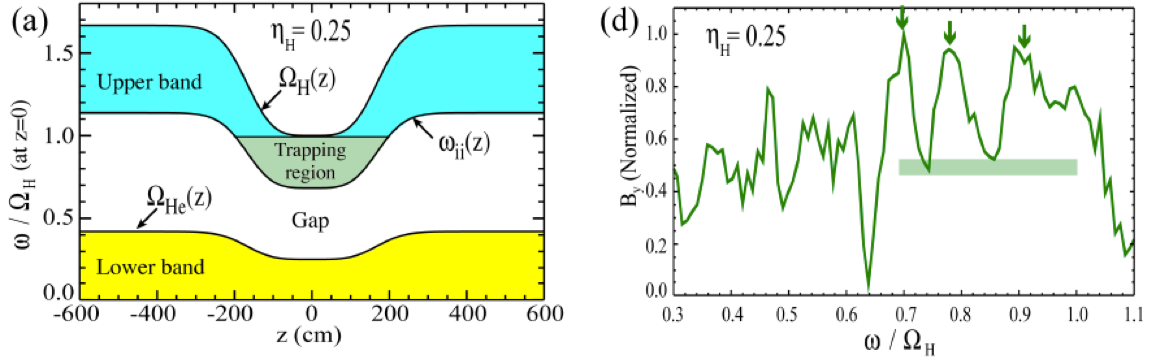
\includegraphics[width=5.0truein]{twoion1}}
\caption{Left: Axial variation of resonator in LAPD for a
H-He\textsuperscript{+} plasma showing propagation bands and gap. Right:
Spectrum of magnetic fluctuations inside resonator shows resonator
peaks; arrows are theoretically-predicted frequencies of trapped
modes.}\label{twoion1}
\end{figure}

\begin{figure}[!htbp]
\centerline{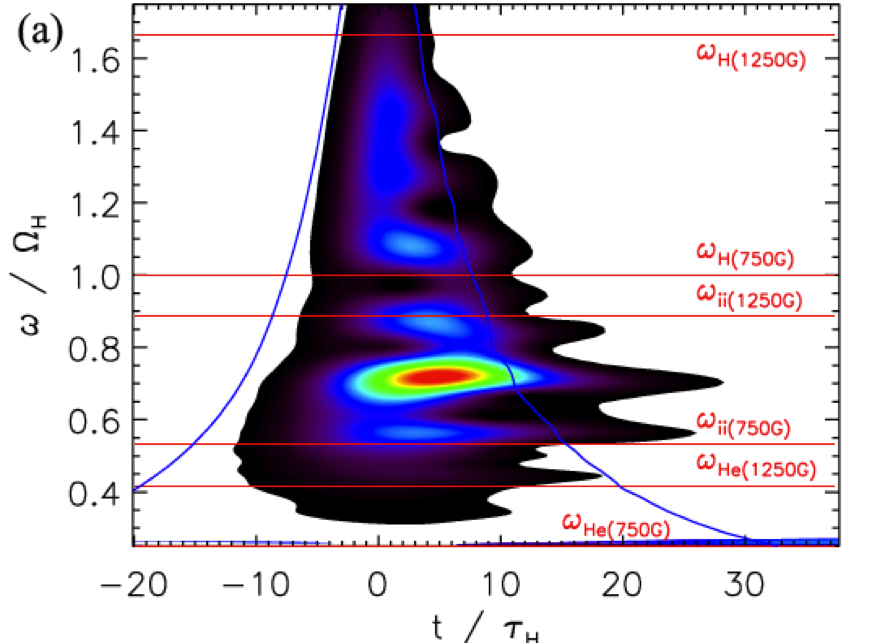
\includegraphics[width=4.4truein]{twoion2}}
\caption{Contours of Morlet wavelet amplitude of magnetic field
fluctuations show the response of the
H\textsuperscript{+}-He\textsuperscript{+} resonator after excitation
with a current impulse of width $\Delta t = \tau_H$ at
$t = 0$. Red spot shows a large response and long lifetime of a
trapped mode.}\label{twoion2}
\end{figure}

This work lead to a Ph.D. dissertation by W. Farmer and has been
reported in seven publications. The most recent effort has used the
insight from the LAPD studies to assess the properties of such a
resonator for the expected ITER environment and its excitation by
energetic alpha particles~\cite{farmer:2014}.


\subsubsection{Magnetic Flux Ropes (W. Gekelman, B. Van Compernolle; E.
Lawrence, T. DeHaas, D. Hong (Graduate Students))}

The UCLA group (W. Gekelman, B. Van Compernolle, and graduate students
past (Eric Lawrence) and present (Tim DeHaas, Dooran Hong) have done
groundbreaking work on the interaction of magnetic flux ropes. We are
presently collaborating with W. Daughton (LANL) on a experiment
dedicated to the memory of Tom Intrator.

The first ever experimental
determination~\cite{lawrence:2009} of a quasi-seperatrix layer
(QSL) was made on the LAPD in 2009. A QSL is a 3D region in which
magnetic field lines that start close to one another diverge rapidly in
space. The value of Q is a measure of the divergence. If two field lines
pass through a reconnection region, one or more components of B can
rapidly change within it leading to a large value of Q. This is
illustrated in Figure~\ref{ropes1}.

\begin{figure}[!htbp]
\centerline{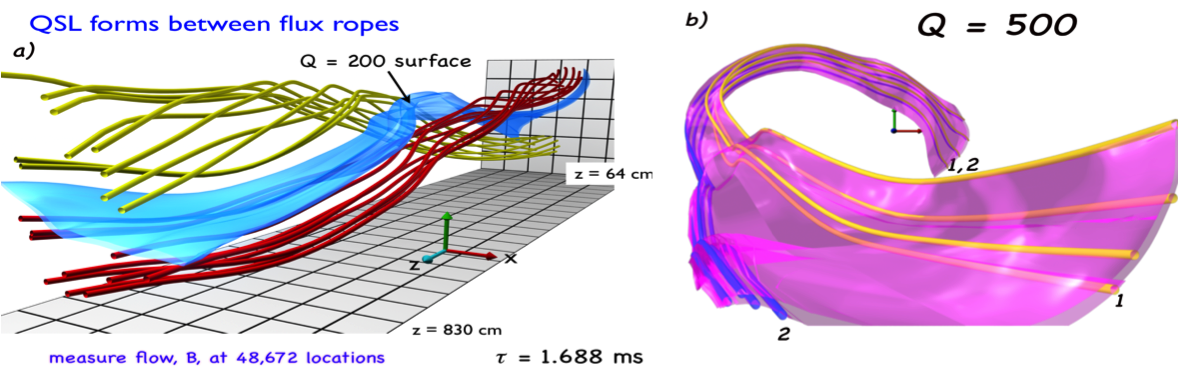
\includegraphics[width=5.0truein]{ropes1}}
\caption{(a) The ``blue'' surface is a QSL (Q=100) which is located
between two flux ropes which are colored red and yellow. The flux ropes
are calculated by following field lines through the dense grid of
measurement points. (b) A Q=500 surface with several field lines
within it. One set of field lines labeled (1,2) are initially 0.5 mm
apart but are 12.5 cm apart when they reach the end of the measurement
volume 8.3 meters away.}\label{ropes1}
\end{figure}

QSLs have been observed in the collision of two or more flux
ropes~\cite{gekelman:2010,vancompernolle:2011}. In a separate tearing mode experiment QSL's
were discovered when 3D current systems expanded in space and no field
line reconnection was involved. For the first time the total electric
field was measured using a
combination of magnetic and emissive probes. The parallel resistivity,
$\eta_\parallel$ was derived from the data and can
be 100's of times the Spitzer resistivity in small regions of space
during the collision of flux ropes. The resistivity was localized to the
gradients in the current of the flux ropes and also within the QSL.
Figure~\ref{ropes2} shows the QSL, current and $\eta_\parallel$
evaluated from the measured plasma current and electric field.

\begin{figure}[!htbp]
\centerline{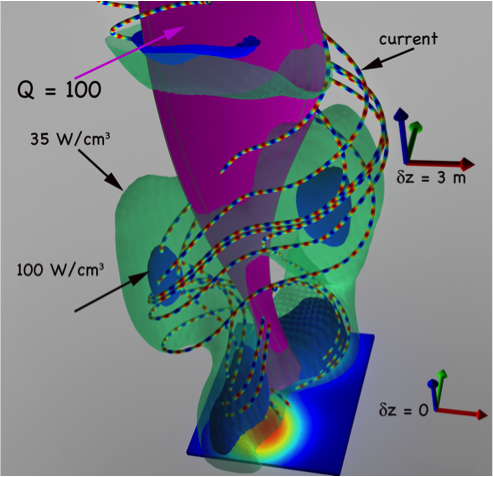
\includegraphics[width=3.4truein]{ropes2}}
\caption{Bottom is the plasma current in a plane 64 cm from the origin
of the ropes. The current of one rope is clearly visible and the current
density in the center is 5A/cm\textsuperscript{2}. A QSL of 100 is shown
along with several current field lines colored in stripes. Two
isosurfaces of the heating power are shown. Heating is observed within
the QSL at locations where reconnection occurs but significant heating
also occurs within the flux tubes.}\label{ropes2}
\end{figure}


It is clear that there is more than one process at work. The three
dimensional case is very different from the traditional 2D models which
cannot predict the reconnection rate we measured by integrating the
electric field along magnetic field lines.

We have also studied chaos associated with the ropes and
found that it peaks when the flux ropes exist along with shear Alfvén
waves~\cite{gekelman:2014}. When the BaO cathode is replaced with a LaB\textsubscript{6}
cathode we will be able to do these experiments are relatively high
plasma beta and Lundquist number
(10\textsuperscript{5} \textless{} L \textless{}10\textsuperscript{6}).
How do intense Alfvén waves interact with flux ropes (which can also be
thought of as Alfvén waves)? What is the mechanism for this interaction
and can it lead to magnetic turbulence? The LAPD is the only machine in
which these experiments can be performed.

\emph{Turbulence, transport and flows in LAPD} (T. Carter, J. Maggs, P.
Popovich (UCLA) M. Umansky (LLNL), B. Dudson (U. York); D. Schaffner, B.
Friedman, G. Rossi (grad students))

Turbulence in magnetically confined plasmas is often attributed to
linear instabilities, which can grow from infinitesimal initial
perturbations (e.g. thermal noise). However, it is well known in the
hydrodynamics community that linear instability (normal mode) analysis
fails at predicting turbulent onset for a number of physical situations,
for example water flow in cylindrical pipes (Poiseuille flow). In these
cases, turbulence arises even though all linear modes are stable,
meaning infinitesimal perturbations on the laminar state cannot grow
exponentially. Nevertheless, finite amplitude perturbations can still
excite turbulence. We have found that the same can be true in
pressure-gradient-driven turbulence in magnetic confinement devices.
This fact makes prediction of turbulence and turbulent transport in
fusion experiments difficult as linear instability calculations, which
are relied on quite heavily in the fusion community, can be misleading.
Using input from analysis of massively-parallel simulations of
turbulence in the Large Plasma Device at UCLA, we developed a technique
that enables the prediction of the nonlinear properties of a turbulent
system using simple linear, but ``nonmodal'', calculations. The
technique successfully predicts the structure of the nonlinearly
saturated state in LAPD turbulence simulations and provide a linear
technique to estimate turbulent saturated amplitude and particle
transport {[}B. Friedman and T.A. Carter, Physical Review Letters 113,
025003 (2014){]}.

More here\ldots{}


\section{Facility Development}

Since its inception, the BaPSF has continually improved the capabilities
and diagnostics of the LAPD device. In the next funding period, among
other improvements, we propose one major upgrade to the LAPD. This
upgrade will replace the primary plasma source, currently a large-area
Barium Oxide emissive cathode, with a Lanthanum Hexaboride (LaB6) based
cathode. Large area LaB6 cathodes have been developed over the last
funding period by the UCLA group (see the appendix for more details) and
offer many advantages to BaO cathodes. BaO cathodes are sensitive to
Oxygen; any significant exposure to Oxygen will ``poison'' the cathode,
substantially lowering its emission. For this reason, any unintentional
vacuum leak leads to an extended shutdown: it takes around 10 days to
replace a poisoned cathode (cathode must be removed, cleaned, re-coated
and slowly ``converted'' while heated under vacuum before it is ready to
be operated). In addition, the introduction of apparatus into the vacuum
chamber in order to perform experiments (e.g. probes or antennas) must
be done very carefully. New apparatus is pumped down to 5x10\^{}-6 Torr
prior to being opened and inserted into the vacuum chamber to prevent
Oxygen from being introduced. For typical probes it can take 2 hours to
achieve this level of vacuum and it can take up to a day of pumping for
larger items (e.g. large antennas). The efficiency of gathering data
using LAPD is therefore reduced by time waiting to open new probes (e.g.
after moving a probe to a new axial location). LaB6 cathodes are far
more robust and do not suffer from the same sensitivity to vacuum
incidents. Using LaB6 for the primary LAPD cathode will therefore
increase uptime and increase efficiency of data taking during the
typical run week. Probes and antennas will need to be evacuated before
insertion into LAPD, but the base pressure required before opening will
be increased, significantly reducing the time to move a probe or
introduce a new antenna.

More importantly, LaB6 cathodes offer far more emission current density,
and therefore higher density and temperature plasmas, than BaO cathodes.
Recently, a 20cm LaB6 cathode has been installed on LAPD (see appendix),
allowing for the production of high density and temperature ``core''
plasmas within the larger BaO-produced plasma. Plasmas are produced with
significantly higher density (up a factor of 50 from BaO to 5x10\^{}13
/cc) and higher electron temperature (up to 12-15 eV from 5-10 eV with
BaO). At this electron density and temperature, the ion-electron
collisional energy exchange time is calculated to be
\$\textbackslash{}sim 0.2\$\textasciitilde{}ms and, consistent with
this, an increased ion temperature is observed in the new LaB\$\_6\$
produced plasma. Initial measurements of shape of the He II
468.6\textasciitilde{}nm ion emission line have been performed using a
2\textasciitilde{}m spectrometer. These measurements have been compared
to PrismSPECT Spectral Analysis Code calculations yielding a best-fit
temperature of \$T\_i \textbackslash{}sim 5\$\textasciitilde{}eV, a
significant enhancement over the BaO produced plasma ion temperature of
\$T\_i \textless{} 1\$\textasciitilde{}eV. {[}Figure to be added{]} The
achievement of a factor of 100x increase in plasma pressure along with
warm ions allows:


\begin{itemize}
\item
  Achievement of high-beta, magnetized plasmas (turbulence and transport
  at high beta, wave physics at high beta, instabilities (mirror and
  firehose)
\item
  Study of kinetic ion physics (Landau, Barnes and Cyclotron damping)
\item
  Studies in a regime with similar density to tokamak boundary plasmas
  (turbulence, RF, etc)
\end{itemize}


{[}This will be expanded{]}

\section{Proposed Research - Local Group}


\subsection{Research on Three Dimensional Current Systems and Magnetic Field
Line Reconnection (W. Gekelman, B. Van Compernolle)}

The UCLA group (W. Gekelman, B. Van Compernolle, graduate students and
external users: W. Daughton (LANL), will continue their successful
program on 3D reconnection. Much of the past work has centered on
reconnection in systems of magnetic flux ropes. The first ever
experimental determination~\cite{lawrence:2009} of a quasi-seperatrix
layer (QSL) was made on the LAPD in 2009. A QSL is a 3D region in
which magnetic field lines that start close to one another diverge
rapidly in space. The value of Q is a measure of the divergence.  If
two field lines pass through a reconnection region, one or more
components of B can rapidly change within it leading to a large value
of Q. This has been seen in the collision of two or more flux
ropes~\cite{gekelman:2010}. In a separate tearing mode experiment
QSL's were discovered when 3D current systems expanded in space and no
field line reconnection was involved. For the first time the total
electric field was measured using a combination of magnetic and
emissive probes. The parallel resistivity was derived from the data
and can be 100's of times the Spitzer resistivity in small regions of
space during the collision of flux ropes. The resistivity was
localized to the gradients in the current of the flux ropes and also
within the QSL. It is clear that there is more than one process at
work. The three dimensional case is very different from the
traditional 2D models which cannot predict the reconnection rate we
measured by integrating the electric field along magnetic field
lines. We have also studied chaos associated with the
ropes and found that it peaks when the
flux ropes exist along with shear Alfvén waves~\cite{gekelman:2014}.

We will continue to explore the nature of 3D current systems and
reconnection in future experiments. What are all the instabilities that
give rise to large plasma resistivity's. Are high frequency waves
involved? With the planned replacement of the BaO cathode we will be
able to do these experiments are relatively high plasma beta and Lundquist number
(10\textsuperscript{5} \textless{} L \textless{}10\textsuperscript{6}).
How do intense Alfvén waves interact with flux ropes (which can also be
thought of as Alfvén waves)? What is the mechanism for this interaction
and can it lead to magnetic turbulence? The LAPD is the only machine in
which these experiments can be done. We look forward to continued
collaboration with the Los Alamos group as well with others interested
in this topic.

\subsection{Avalanche phenomena in magnetized plasmas (B. Van Compernolle, G.
Morales)}

Avalanches are sudden events that cause major changes over an extended
region of a physical system. The origin of avalanches is the presence of
a steep gradient in one of the system parameters. Often there is a
threshold value for the gradient; when it is exceeded, a complex
sequence of processes is triggered whose role is to relax the gradient
below the threshold value. In several environments, such as an
externally-heated or fueled plasma, the sources reestablish the gradient
and further cause it to exceed the threshold value. A sequence of
avalanches can then occur, but the actual time of appearance of an
individual event displays a marked degree of unpredictability. The
behavior is intermittent and causes the parameters of the system to
evolve from place to place, i.e., there is an associated ``transport''
that occurs. It is this type of intermittent avalanche phenomena that
will form the central theme of the proposed studies.

The project will focus on avalanches triggered by gradients in plasma
temperature and density across the magnetic field. This is a situation
encountered in natural plasmas (e.g., sun, earth's magnetotail) and in
fusion devices. The technological breakthrough that makes possible the
implementation of an ideal basic configuration for studies of avalanches
in magnetized plasmas is a reliable and flexible LaB\textsubscript{6}
cathode source that has been developed in BaPSF.

Preliminary results demonstrating the controlled generation of
avalanches using a ring-shaped heat source have been recently
published~\cite{vancompernolle:2015b}. In the near future a full
characterization of cross-field avalanches will be made using the
diagnostic tools available at the LAPD laboratory. Detailed spatial
and temporal measurements of density, temperature, plasma potential,
flows (both ExB and diamagnetic), and magnetic fields, will be
undertaken for a wide range of parameter values, including: heating
power, strength of confinement magnetic field, neutral gas
fill-pressure and ionic species.. The steepness of the pressure
gradient can be adjusted by changing the heating power, which
determines the peak electron temperature within the hot ring. Although
the preliminary results were performed with a constant bias voltage
applied to the LaB\textsubscript{6} source, a straightforward
extension is to control, and change, the bias voltage during the
experiment. This capability permits the identification of various
features, such as hysteresis and response to modulations of the
critical gradient.

In summary, the wide range of experimental capabilities at BaPSF allows
for the investigation of a number of important questions related to
avalanches in magnetized plasmas including

quantitative information about SOC dynamics, the formation and evolution
of streamers, the effects of flows, the connection between avalanches
and 'blobs', and the role of nonlocal transport of both temperature and
density during avalanche events.


\subsection{Turbulence and Transport (T.
Carter, F. Jenko)}

{[}place holder text{]} The proposed research aims at studying the
fundamental physics of pressure-gradient-driven instabilities and
associated turbulence and transport in an experiment where the
\$\textbackslash{}beta\$ value can be varied over several orders of
magnitude, from \$\textbackslash{}beta\textbackslash{}sim 10\^{}\{-4\}\$
to \$\textbackslash{}beta\textbackslash{}sim 1\$. The work is enabled by
a the new secondary LaB6 plasma source that can create plasmas with
significantly increased thermal energy density, which, along with the
ability to vary the magnetic field while keeping the plasma magnetized,
allows

for accessing a wide range of \$\textbackslash{}beta\$ values. In
addition, the production of warm ions provides an opportunity to
investigate ion kinetic effects on the turbulence. In the proposed work,
focus will

be given to a detailed, quantitative study of the response of
turbulence, turbulent transport, and spontaneously generated flows to
variation of \$\textbackslash{}beta\$. Existing capabilities to
externally control flow and flow shear will be used to extend previous
work on the suppression of particle transport by flow shear to higher
\$\textbackslash{}beta\$ regimes. Finally, we will undertake work to
make a very important further development regarding the capability to
simulate LAPD plasmas, including kinetic effects. The state-of-the-art
gyrokinetic turbulence code GENE, capable of handling high
\$\textbackslash{}beta\$ electromagnetic effects, will be used for
simulation studies of LAPD plasmas. These will be the first global ab
initio computations of LAPD plasmas, allowing to carry out
simulation-experiment comparisons in the high \$\textbackslash{}beta\$
regime with unprecedented quality.

\subsection{Physics of Compressional Alfven waves in LAPD (Vincena, Tripathi,
Van Compernolle, Carter)}

{[}To be added{]}


\section{Future Campaign Development}

The topical campaign has been an extremely successful operating mode and
will continue to be emphasized in the next funding cycle. The
development of new campaigns will proceed in consultation with the BaPSF
council and through interaction with members of the research community.
Support is requested to run workshops at UCLA (roughly every other year)
to support the development and operation of campaigns. Here are
presented several possible research topics that could be the subject of
future campaigns; actual

a). \emph{``Solar Wind'' Campaign.} Alfvénic turbulence is observed
directly in the solar wind, indirectly in the interstellar medium and is
thought to play an important role in momentum transport and heating in
accretion disks; a campaign in this area could have a major impact. Such
a campaign would build on existing efforts, including initial Alfvén
single wave-wave interaction studies on LAPD47 and detailed comparisons
between astrophysical turbulence simulation codes and LAPD data48.
Possible near term activities in such a campaign could include extension
of Alfvén wave studies to high beta in LAPD using a LaB6 plasma source
and studies of high-beta anisotropy driven instabilities such as the
mirror or firehose instability, both thought to be very important in
establishing the turbulent spectrum and heating in turbulence at high
beta. Greg Howes (U. Iowa) has agreed to help lead this campaign.
{[}More to be added{]}

b)\emph{. RF Physics Campaign.} A campaign proposal that has already
been under development is the study of the basic physics of
radiofrequency (RF) waves for heating and current drive. R. Perkins
(PPPL) has expressed interest in coordinating a campaign on fast wave
physics, in particular focused on interaction with edge plasmas and the
generation of RF sheaths. Initial research focus would be placed on RF
sheaths driven by fast wave antennas in an attempt to understand RF
sheaths and validate models used in fusion RF codes. Impurity production
associated with RF-sheath-driven sputtering is a key issue for ITER
{[}45{]}.


{[}Add more here, discussing Helicon current drive physics and potential
involvement from GA (Pinsker){]}


\section{Intellectual Merit.}

The BaPSF allows the detailed study, under controlled conditions, of
fundamental questions in plasma science that cannot be addressed in any
other laboratory. The results obtained impact a wide range of frontier
topics in fusion and space plasma research. It also lays the foundation
for future developments in plasma technology. Through creative
developments of plasma sources and the operation of complementary plasma
devices exploited thorough focused campaigns, the operation of BaPSF

constitutes a transformative concept within plasma science.

\section{Broader Impacts.}

One of the broader impacts of the BaPSF is that it provides unique
opportunities in the training of young researchers from both large and
small institutions. Graduate students, postdoctoral researchers and
assistant professors have access to cutting edge research devices
without the burden of maintenance. The ideal mid-scale size of the
devices allows for individual creativity to blossom within a team
research environment that mixes young students with distinguished senior
researchers. BaPSF fosters and engenders collaborations between domestic
and international institutions and scientists from diverse

areas, such as fusion, space and industrial applications. The topical
campaigns made possible by BaPSF provides a forum for the interaction of
experimentalists, theoreticians and modelers from varied backgrounds,
promoting the cross-fertilization of ideas and techniques. Research at
BaPSF is published over a wide range of refereed journals and is
presented extensively at prestigious national and international
conferences covering all aspects of plasma science. The LAPTAG program
run by the facility also provides research opportunities for high school
students and teachers.


\newpage

\setcounter{page}{1}

%\bibliographystyle{unsrtnat}
%\bibliographystyle{prsty}
\bibliographystyle{unsrt}
\bibliography{refs}  




\end{document}
